\documentclass{article}
\usepackage{listings}
\usepackage{graphicx}
\usepackage{color}

\definecolor{mygreen}{rgb}{0,0.6,0}
\definecolor{mygray}{rgb}{0.5,0.5,0.5}
\definecolor{mymauve}{rgb}{0.58,0,0.82}

\lstset{ %
  backgroundcolor=\color{white},   % choose the background color; you must add \usepackage{color} or \usepackage{xcolor}; should come as last argument
  basicstyle=\footnotesize,        % the size of the fonts that are used for the code
  breakatwhitespace=false,         % sets if automatic breaks should only happen at whitespace
  breaklines=true,                 % sets automatic line breaking
  captionpos=b,                    % sets the caption-position to bottom
  commentstyle=\color{mygreen},    % comment style
  deletekeywords={...},            % if you want to delete keywords from the given language
  escapeinside={\%*}{*)},          % if you want to add LaTeX within your code
  extendedchars=true,              % lets you use non-ASCII characters; for 8-bits encodings only, does not work with UTF-8
  frame=single,	                   % adds a frame around the code
  keepspaces=true,                 % keeps spaces in text, useful for keeping indentation of code (possibly needs columns=flexible)
  keywordstyle=\color{blue},       % keyword style
  language=Octave,                 % the language of the code
  morekeywords={*,...},           % if you want to add more keywords to the set
  numbers=left,                    % where to put the line-numbers; possible values are (none, left, right)
  numbersep=5pt,                   % how far the line-numbers are from the code
  numberstyle=\tiny\color{mygray}, % the style that is used for the line-numbers
  rulecolor=\color{black},         % if not set, the frame-color may be changed on line-breaks within not-black text (e.g. comments (green here))
  showspaces=false,                % show spaces everywhere adding particular underscores; it overrides 'showstringspaces'
  showstringspaces=false,          % underline spaces within strings only
  showtabs=false,                  % show tabs within strings adding particular underscores
  stepnumber=2,                    % the step between two line-numbers. If it's 1, each line will be numbered
  stringstyle=\color{mymauve},     % string literal style
  tabsize=2,	                   % sets default tabsize to 2 spaces
  title=\lstname                   % show the filename of files included with \lstinputlisting; also try caption instead of title
}

\author{Jacob Hutter, Junhao Pan}
\title{ECE 313 Final Project Report}

\begin{document}
\maketitle


\underline{\textbf{Task 0:}}
\begin{lstlisting}
    clear all;
    clc;

    load 1_a41178.mat;
    patient1_data = floor(all_data);
    patient1_labels = all_labels;
    training1 = patient1_data(:,1:(2*length(patient1_data)/3));
    testing1 = patient1_data(:,(2*length(patient1_data)/3):length(patient1_data));
    label_training1 = patient1_labels(1:(2*length(patient1_labels)/3));
    label_testing1 = patient1_labels((2*length(patient1_labels)/3):length(patient1_labels));

    load 2_a42126.mat;
    patient2_data = floor(all_data);
    patient2_labels = all_labels;
    training2 = patient2_data(:,1:floor(2*length(patient2_data)/3));
    testing2 = patient2_data(:,floor(2*length(patient2_data)/3):length(patient2_data));
    label_training2 = patient2_labels(1:floor(2*length(patient2_labels)/3));
    label_testing2 = patient2_labels(floor(2*length(patient2_labels)/3):length(patient2_labels));

    load 3_a40076.mat;
    patient3_data = floor(all_data);
    patient3_labels = all_labels;
    training3 = patient3_data(:,1:(2*length(patient3_data)/3));
    testing3 = patient3_data(:,(2*length(patient3_data)/3):length(patient3_data));
    label_training3 = patient3_labels(1:(2*length(patient3_labels)/3));
    label_testing3 = patient3_labels((2*length(patient3_labels)/3):length(patient3_labels));

    load 4_a40050.mat;
    patient4_data = floor(all_data);
    patient4_labels = all_labels;
    training4 = patient4_data(:,1:floor(2*length(patient4_data)/3));
    testing4 = patient4_data(:,floor(2*length(patient4_data)/3):length(patient4_data));
    label_training4 = patient4_labels(1:floor(2*length(patient4_labels)/3));
    label_testing4 = patient4_labels(floor(2*length(patient4_labels)/3):length(patient4_labels));

    load 5_a41287.mat;
    patient5_data = floor(all_data);
    patient5_labels = all_labels;
    training5 = patient5_data(:,1:(2*length(patient5_data)/3));
    testing5 = patient5_data(:,(2*length(patient5_data)/3):length(patient5_data));
    label_training5 = patient5_labels(1:(2*length(patient5_labels)/3));
    label_testing5 = patient5_labels((2*length(patient5_labels)/3):length(patient5_labels));

    load 6_a41846.mat;
    patient6_data = floor(all_data);
    patient6_labels = all_labels;
    training6 = patient6_data(:,1:floor(2*length(patient6_data)/3));
    testing6 = patient6_data(:,floor(2*length(patient6_data)/3):length(patient6_data));
    label_training6 = patient6_labels(1:floor(2*length(patient6_labels)/3));
    label_testing6 = patient6_labels(floor(2*length(patient6_labels)/3):length(patient6_labels));

    load 7_a41846.mat;
    patient7_data = floor(all_data);
    patient7_labels = all_labels;
    training7 = patient7_data(:,1:floor(2*length(patient7_data)/3));
    testing7 = patient7_data(:,floor(2*length(patient7_data)/3):length(patient7_data));
    label_training7 = patient7_labels(1:floor(2*length(patient7_labels)/3));
    label_testing7 = patient7_labels(floor(2*length(patient7_labels)/3):length(patient7_labels));

    load 8_a42008.mat;
    patient8_data = floor(all_data);
    patient8_labels = all_labels;
    training8 = patient8_data(:,1:(2*length(patient8_data)/3));
    testing8 = patient8_data(:,(2*length(patient8_data)/3):length(patient8_data));
    label_training8 = patient8_labels(1:(2*length(patient8_labels)/3));
    label_testing8 = patient8_labels((2*length(patient8_labels)/3):length(patient8_labels));

    load 9_a41846.mat;
    patient9_data = floor(all_data);
    patient9_labels = all_labels;
    training9 = patient9_data(:,1:floor(2*length(patient9_data)/3));
    testing9 = patient9_data(:,floor(2*length(patient9_data)/3):length(patient9_data));
    label_training9 = patient9_labels(1:floor(2*length(patient9_labels)/3));
    label_testing9 = patient9_labels(floor(2*length(patient9_labels)/3):length(patient9_labels));
\end{lstlisting}
For task 0 we took the raw patient and gold data and partitioned it into testing and training segments.
\\ \underline{\textbf{Task 1.1:}}
\begin{lstlisting}
HT_table_array_pat_1 = Get_HT_table(1, training1, label_training1);
HT_table_array_pat_2 = Get_HT_table(2, training2, label_training2);
HT_table_array_pat_3 = Get_HT_table(3, training3, label_training3);
HT_table_array_pat_4 = Get_HT_table(4, training4, label_training4);
HT_table_array_pat_5 = Get_HT_table(5, training5, label_training5);
HT_table_array_pat_6 = Get_HT_table(6, training6, label_training6);
HT_table_array_pat_7 = Get_HT_table(7, training7, label_training7);
HT_table_array_pat_8 = Get_HT_table(8, training8, label_training8);
HT_table_array_pat_9 = Get_HT_table(9, training9, label_training9);

HT_table_array = cat(1, HT_table_array_pat_1, HT_table_array_pat_2, HT_table_array_pat_3, HT_table_array_pat_4, HT_table_array_pat_5, HT_table_array_pat_6, HT_table_array_pat_7, HT_table_array_pat_8, HT_table_array_pat_9);
\end{lstlisting}
\begin{lstlisting}
function HT_table_array_pat = Get_HT_table(patient_index, patient_data, patient_labels)

% Prior probablities, alarms/total
P_H1 = sum(patient_labels)/length(patient_labels);
P_H0 = 1 - P_H1;

HT_table_array_pat = cell(1, 7);

% name = strcat('Patient_', int2str(patient_index), '_Features');
% figure('name', name, 'unit', 'normalized', 'outerposition', [.1 .1 .8 .8]);

for i = 1:7
	[feature_mat, x_mat] = Get_Feat_Mat(patient_data(i:i, :), patient_labels);

	ML_vector = zeros(1, length(feature_mat(1:1, :)));
	MAP_vector = zeros(1, length(feature_mat(1:1, :)));

	for k = 1:length(feature_mat(1:1, :))
		P_H1_i = feature_mat(1, k);
		P_H0_i = feature_mat(2, k);
		if (P_H1_i >= P_H0_i)
			% if H1_pmf >= H0_pmf
			ML_vector(k) = 1;
		end
		if (P_H1*P_H1_i >= P_H0*P_H0_i)
			% if H1_pmf*P(H1) >= H0_pmf*P(H0)
			MAP_vector(k) = 1;
		end
	end

	HT_table = cat(1, x_mat, feature_mat(1:1, :), feature_mat(2:2, :), ML_vector, MAP_vector);
	HT_table = rot90(HT_table, -1);
	HT_table = fliplr(HT_table);
	% Have to flip the table so that it matches with the given format
	HT_table_array_pat{1, i} = num2cell(HT_table);
	subplot(7, 1, i);
 	hold on;
 	plot(x_mat, feature_mat(1:1, :));
 	plot(x_mat, feature_mat(2:2, :));
 	legend('H0 pmf', 'H1 pmf');
 	hold off;
end
\end{lstlisting}
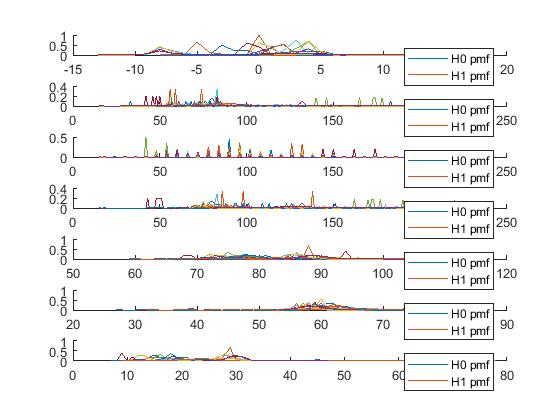
\includegraphics[scale = 0.7]{untitled}
\\Above is our data after we created the probability matricies.
\underline{\textbf{Task 1.2:}}
\begin{lstlisting}
  Error_table_arrar_pat_1 = Get_Error_table(HT_table_array_pat_1, testing1, label_testing1);
  Error_table_arrar_pat_2 = Get_Error_table(HT_table_array_pat_2, testing2, label_testing2);
  Error_table_arrar_pat_3 = Get_Error_table(HT_table_array_pat_3, testing3, label_testing3);
  Error_table_arrar_pat_4 = Get_Error_table(HT_table_array_pat_4, testing4, label_testing4);
  Error_table_arrar_pat_5 = Get_Error_table(HT_table_array_pat_5, testing5, label_testing5);
  Error_table_arrar_pat_6 = Get_Error_table(HT_table_array_pat_6, testing6, label_testing6);
  Error_table_arrar_pat_7 = Get_Error_table(HT_table_array_pat_7, testing7, label_testing7);
  Error_table_arrar_pat_8 = Get_Error_table(HT_table_array_pat_8, testing8, label_testing8);
  Error_table_arrar_pat_9 = Get_Error_table(HT_table_array_pat_9, testing9, label_testing9);

  Error_table_arrar = cat(1, Error_table_arrar_pat_1, Error_table_arrar_pat_2, Error_table_arrar_pat_3, Error_table_arrar_pat_4, Error_table_arrar_pat_5, Error_table_arrar_pat_6, Error_table_arrar_pat_7, Error_table_arrar_pat_8, Error_table_arrar_pat_9);

  \end{lstlisting}
  \begin{lstlisting}
    function Error_table_pat = Get_Error_table(HT_table_array_pat, patient_data, patient_labels)

    Error_table_pat = cell(1, 7);

    for i = 1:7
        % Get feature from the parameter
    	feature_table = HT_table_array_pat{1, i};
        feature_data = patient_data(i:i, :);
        % Offset the data
    	feature_data_off = feature_data - min(feature_data) + 1;

        % Get the vectors and organize
    	ML_vector = cell2mat(feature_table(:, 4:4));
    	MAP_vector = cell2mat(feature_table(:, 5:5));
    	ML_vector = rot90(ML_vector);
    	MAP_vector = rot90(MAP_vector);
        ML_vector_off = zeros(1, max(feature_data_off));
    	MAP_vector_off = zeros(1, max(feature_data_off));
    	for k = 1:length(ML_vector)
    		ML_vector_off(k) = ML_vector(k);
    		MAP_vector_off(k) = MAP_vector(k);
        end

        % Alarms generated by vectors
        ML_vector_alarm = zeros(1, length(patient_labels));
    	MAP_vector_alarm = zeros(1, length(patient_labels));
    	for k = 1:length(feature_data_off)
    		j = feature_data_off(k);
    		if (ML_vector_off(j) == 1)
    			ML_vector_alarm(k) = 1;
    		end
    		if (MAP_vector_off(j) == 1)
    			MAP_vector_alarm(k) = 1;
    		end
        end

        % count the errors
    	FA_count_ML = 0;
    	MD_count_ML = 0;
    	FA_count_MAP = 0;
    	MD_count_MAP = 0;
    	for k = 1:length(patient_data)
    		if (patient_labels(k) == 1)
    			if (ML_vector_alarm(k) == 0)
    				MD_count_ML = MD_count_ML + 1;
    			end
    			if (MAP_vector_alarm(k) == 0)
    				MD_count_MAP = MD_count_MAP + 1;
    			end
    		else
    			if (ML_vector_alarm(k) == 1)
    				FA_count_ML = FA_count_ML + 1;
    			end
    			if (MAP_vector_alarm(k) == 1)
    				FA_count_MAP = FA_count_MAP + 1;
    			end
    		end
        end

        % Contruct the error table
        Error_table = zeros(2, 3);
    	number_alarm = sum(patient_labels);
    	total_alarm = length(patient_labels);
    	Error_table(1, 1) = FA_count_ML/(total_alarm - number_alarm);
    	Error_table(1, 2) = MD_count_ML/number_alarm;
    	Error_table(1, 3) = (FA_count_ML + MD_count_ML)/total_alarm;
    	Error_table(2, 1) = FA_count_MAP/(total_alarm - number_alarm);
    	Error_table(2, 2) = MD_count_MAP/number_alarm;
    	Error_table(2, 3) = (FA_count_MAP + MD_count_MAP)/total_alarm;
    	Error_table_pat{1, i} = num2cell(Error_table);
    end
    \end{lstlisting}
    Above you can see we created the Ml and map rule errors for the matrix.

  \\  \underline{\textbf{Task 2.1:}}
  \begin{lstlisting}
  patient_data_array = cell(1, 9);
  patient_data_array{1, 1} = num2cell(patient1_data);
  patient_data_array{1, 2} = num2cell(patient2_data);
  patient_data_array{1, 3} = num2cell(patient3_data);
  patient_data_array{1, 4} = num2cell(patient4_data);
  patient_data_array{1, 5} = num2cell(patient5_data);
  patient_data_array{1, 6} = num2cell(patient6_data);
  patient_data_array{1, 7} = num2cell(patient7_data);
  patient_data_array{1, 8} = num2cell(patient8_data);
  patient_data_array{1, 9} = num2cell(patient9_data);

  corrcoef_array = cell(9, 9, 7);
  for i = 1:7
      for m = 1:9
          for n = 1:9
              patient_data_m = cell2mat(patient_data_array{1, m});
              patient_data_n = cell2mat(patient_data_array{1, n});
              feature_table_m = patient_data_m(i:i, :);
              feature_table_n = patient_data_n(i:i, :);
              % Can't corrcoef if dimensions are different
              % Expand the array by adding a zero to the right position
              array_size = max(length(feature_table_m), length(feature_table_n));
              feature_table_m(array_size) = 0;
              feature_table_n(array_size) = 0;
              corr_coef = corrcoef(feature_table_m, feature_table_n);
              corrcoef_array{m, n, i} = corr_coef(1, 2);
          end
      end
  end
  \end{lstlisting}
  \\ Essentially for 2.1 we iterated through every possibility of patient and feature combination to see that the correlation between patient 6 and patient 9 is always 1 so they have the same data.

  \\  \underline{\textbf{Task 2.2:}}
  \begin{lstlisting}
    feat1,feat2] = find_lowest_eror(Error_table_arrar); % find possible features using addition of errors
    [feat3,feat4] = find_lowest_corr(training1,training2,training3,training4,training5,training6,training7,training8,training9);
    % after the 2 data analysis runs, we have feat1 = 5, feat2 = 7, feat3 = 2,
    % feat4 = 7. the pair 5&7 has a error sum of 5: 2.2, 7:2.4, and a
    % correlation magnitude of .8346 which is terrrible. while the error sum of
    % 2: 3.6 is not terrible and the correlation of 2 and 7 is at a minimum of
    % the set at .0192
  \end{lstlisting}

  \begin{lstlisting}
    function [ feature1,feature2 ] = find_lowest_eror( error_arr )

        local_error = 0;
        global_error = 1000000;
        global_error2 = 1000000;
        local_feat1 = 0;
        local_feat2 = 0;
        for i=1:7
            for j=1:9
                cel = error_arr{j,i};
                error_feature = cel{1,3} + cel{2,3}; % sum up error for that feature in that patient
                local_error = local_error + error_feature; % add to local sum and move to next patient
            end
            if(local_error <= global_error)
                global_error = local_error;
                local_feat2 = local_feat1;
                local_feat1 = i;
            else
                if(local_error <= global_error2)
                    global_error2 = local_error;
                    local_feat2 = i;
                end

            end
            local_error = 0;
        end


        feature1 = local_feat1;
        feature2 = local_feat2;

    end


    \end{lstlisting}
  \begin{lstlisting}
    function [ feature1,feature2 ] = find_lowest_corr( pat1,pat2,pat3,pat4,pat5,pat6,pat7,pat8,pat9 )
        f1 =  cat(2,pat1(1,:),pat2(1,:),pat3(1,:),pat4(1,:),pat5(1,:),pat6(1,:),pat7(1,:),pat8(1,:),pat9(1,:));
        f2 =  cat(2,pat1(2,:),pat2(2,:),pat3(2,:),pat4(2,:),pat5(2,:),pat6(2,:),pat7(2,:),pat8(2,:),pat9(2,:));
        f3 =  cat(2,pat1(3,:),pat2(3,:),pat3(3,:),pat4(3,:),pat5(3,:),pat6(3,:),pat7(3,:),pat8(3,:),pat9(3,:));
        f4 =  cat(2,pat1(4,:),pat2(4,:),pat3(4,:),pat4(4,:),pat5(4,:),pat6(4,:),pat7(4,:),pat8(4,:),pat9(4,:));
        f5 =  cat(2,pat1(5,:),pat2(5,:),pat3(5,:),pat4(5,:),pat5(5,:),pat6(5,:),pat7(5,:),pat8(5,:),pat9(5,:));
        f6 =  cat(2,pat1(6,:),pat2(6,:),pat3(6,:),pat4(6,:),pat5(6,:),pat6(6,:),pat7(6,:),pat8(6,:),pat9(6,:));
        f7 =  cat(2,pat1(7,:),pat2(7,:),pat3(7,:),pat4(7,:),pat5(7,:),pat6(7,:),pat7(7,:),pat8(7,:),pat9(7,:));
        local_min = 0;
        global_min = 10;
        features = [f1;f2;f3;f4;f5;f6;f7]; % make 2d array of feature data for all patients
        for i =1:6
            for j = (i+1):7
               corr = corrcoef(features(i,:),features(j,:)); % should be a 2x2 with flipped entries in each col so just sum column
               local_min = abs(corr(1,2)); % looking for smallest mag of correlation because this fits description better

               if(global_min >= local_min)
                   global_min = local_min;
                   feature1 = i;
                   feature2 = j;
               end
               local_min = 0;
            end
        end
        % concatenate each feature data for each patient;


    end
    \end{lstlisting}
    \\ After examining the output of the two functions and interpreting the data, we were left with the pairs of feature 5 and 7 or 2 and 7. If we analyze the error for each one and the correlation of them, the 2 and 7 pair is much better suited. so we have chosen those two features. However, we can use 5 and 7 for future hypothesis testing because of their low error.

\end{document}
